
Parallel editor is provided as a plugin for the Eclipse integrated development environment. 
Installation can be performed using the built-in mechanism within it or by manually downloading
the plugin files and placing them in the proper plugin folder.

\subsubsection{Installation within Eclipse}

\begin{enumerate}
\item
  Select \emph{``Install new software''} under the Eclipse
  \emph{``Help''} menu.

\item
  Click the \emph{``Add''} button in order to add the location of
  Parallel Editor plugin repository.

\item
  Enter http://maurociancio.github.com/parallel-editor/update-site/
  in the location address and click \emph{``Ok''}. You may optionally
  enter a description for the repository.
  
  \begin{figure}[!ht]
	\begin{center}
		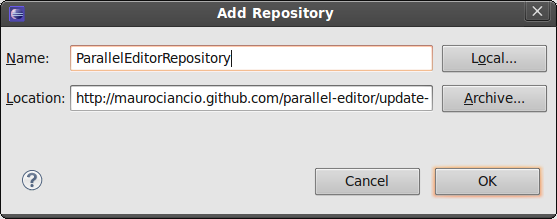
\includegraphics[width=10cm]{addsite.png}
		\caption{\label{addsite} Add Site dialog.}
	\end{center}
  \end{figure}

\item
  You should now see ParallelEditor plugin listed (Fig. \ref{installsoftware}). Select it and
  click \emph{``Next''} 
  \begin{figure}[!ht]
	\begin{center}
		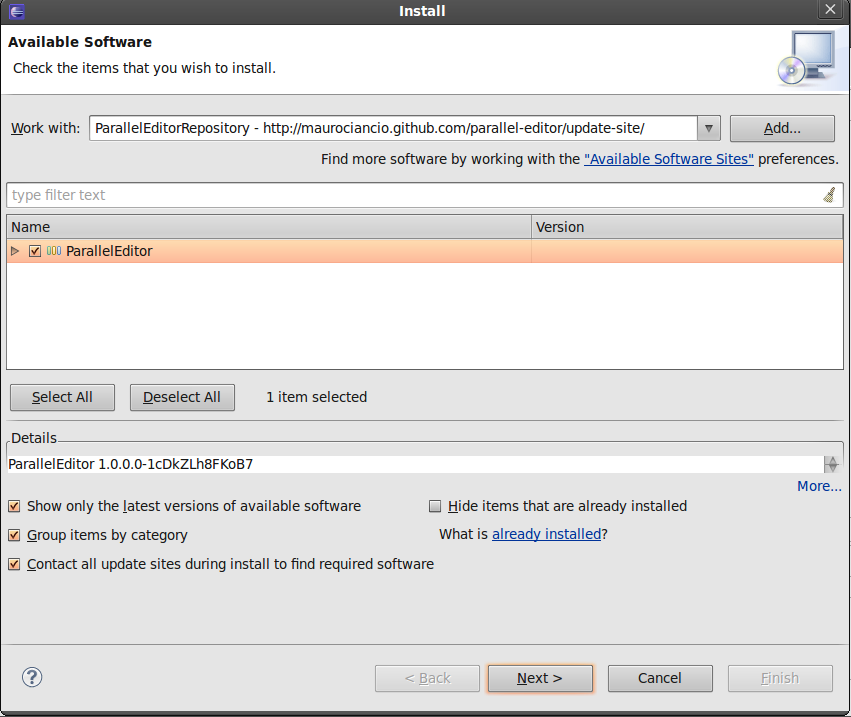
\includegraphics[width=12cm]{installsoftware.png}
		\caption{\label{installsoftware} Install new software dialog.}
	\end{center}
  \end{figure}

\item
  After this step the process is straightforward. Confirm your
  selection, read and accept the license provided if agreed (Fig. \ref{license}) and click
  \emph{``Finish''} to complete the installation.
  \begin{figure}[!ht]
	\begin{center}
		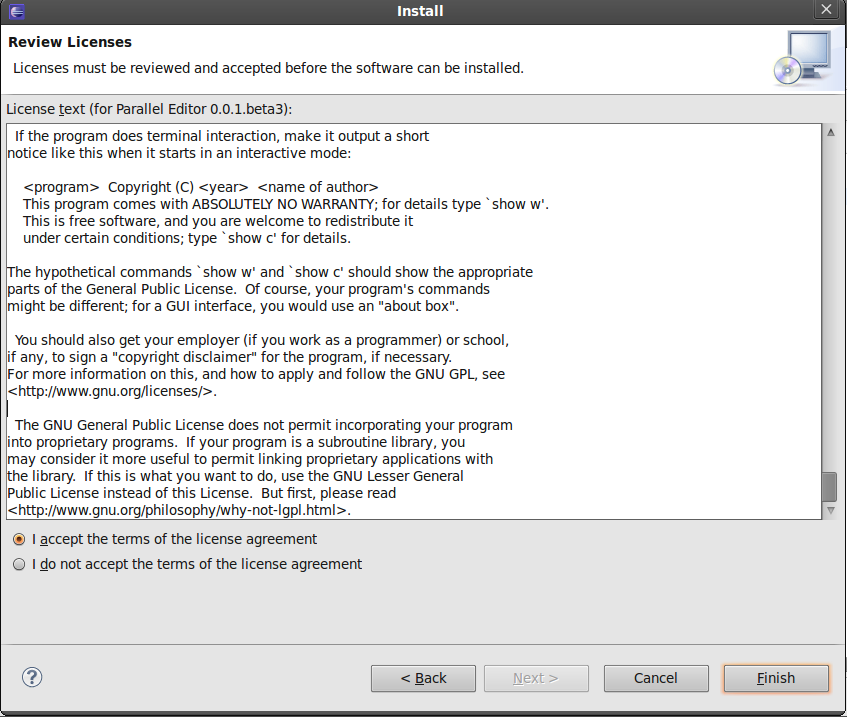
\includegraphics[width=10cm]{licence.png}
		\caption{\label{license} License agreement.}
	\end{center}
  \end{figure}

\end{enumerate}

\subsubsection{Manual installation}

An optional way to install the plugin is available, however this method is not recommended. To perform a manual installation follow these steps.

\begin{enumerate}
\item Clone the project from: \\
\texttt{git://github.com/maurociancio/parallel-editor.git}.
\item Build the plugin dependencies by issuing in your console: "\texttt{mvn clean install}".
\item Use the script in the base folder in order to copy the dependencies to the Eclipse Plugin. Type: \texttt{./copy\_libs\_to\_eclipse\_plugin.sh}.
\item Build the Eclipse Plugin .jar using the Update Site project located in the folder: \texttt{parallel-editor-eclipse-extras}.
\item Place the .jar file generated in your Eclipse plugin folder  (usually /plugins) under the Eclipse installation folder.
\item Restart Eclipse.
\end{enumerate}

ParallelEditor plugin should now be available.

